\documentclass{beamer}

\usepackage{graphicx}
\usepackage{amsmath}
\usepackage{framed}

\begin{document}
	
	% = http://cran.rstudio.com/web/packages/dplyr/vignettes/introduction.html
%===============================================%
\begin{frame}
\begin{figure}
\centering

\includegraphics[width=0.60\linewidth]{dplyr-hexbin-logo}
\end{figure}
\Large
\[ \mbox{Coding Grace 2016 - dplyr}\]
\end{frame}		
	%===============================================%
	\begin{frame}
		\vspace{-0.5cm}
		\LARGE
		\textbf{Overview}
		
		\begin{itemize}
			\item \textbf{dplyr} - data manipulation


			\item \textbf{magrittr} - pipe operator
		\end{itemize}
			\begin{figure}
				\centering
				
\includegraphics[width=0.35\linewidth]{dplyr-hexbin-logo}
				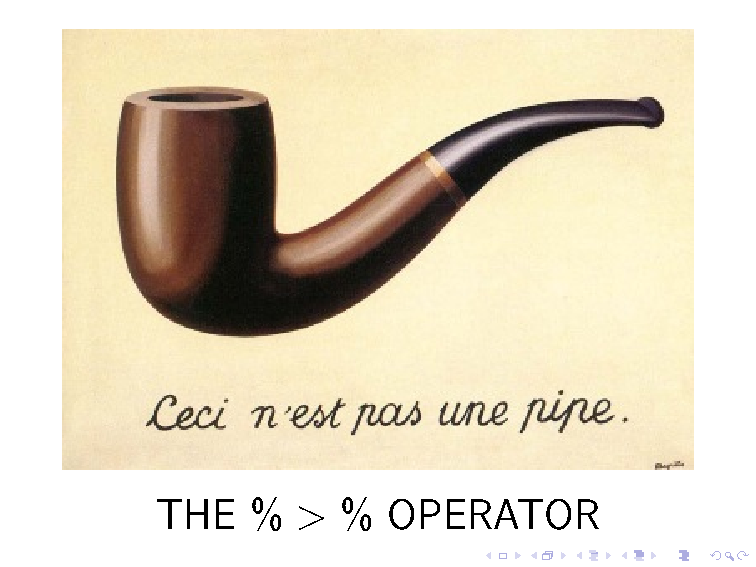
\includegraphics[width=0.35\linewidth]{magrittr}
			\end{figure}	
\end{frame}
	%===============================================%
	\begin{frame}
	\frametitle{Hadley Wickham}
	\begin{figure}
\centering
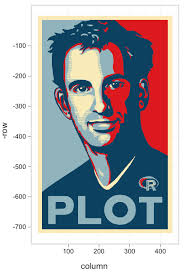
\includegraphics[width=0.5\linewidth]{HWgraphic}
\end{figure}

	\end{frame}

	% If you've used plyr before, many of these will be familar.
	
	\begin{frame}[fragile]
		\frametitle{dplyr : Grammar of data manipulation}
		\Large
		\textbf{What is dplyr?}
		\begin{itemize}
			\item \textbf{dplyr} is mainly authored by Hadley Wickham and Romain Francois. It is designed to be intuitive and easy to learn, thereby making ``doing things" in \texttt{R} more user-friendly.
			\item \textbf{dplyr} is a new package which provides a set of tools for efficiently manipulating datasets in \texttt{R}.
			\item \textbf{dplyr} is the next iteration of plyr, focussing on only data frames. 
			% \item \textbf{dplyr} is faster, has a more consistent API and should be easier to use. 
		\end{itemize}\smallskip
		\textit{(from Hadley Wickham's Vignette)}
	\end{frame}
	%=================================================================== %
	
	\begin{frame}
		\frametitle{dplyr : abstract by Hadley Wickham}	
		\Large
		\textbf{Hadley Wickham's Abstract}\\
		\noindent There are three key ideas that underlie \textbf{dplyr}:
		
		\begin{enumerate}
			\item[1] Your time is important, so Romain Francois has written the key pieces in \textbf{Rcpp} to provide blazing fast performance. \\ \bigskip Performance will only get better over time, especially once we figure out the best way to make the most of multiple processors. 
		\end{enumerate}
	\end{frame}
	%========================================================== %
	\begin{frame}
		\frametitle{dplyr : abstract by Hadley Wickham}	
		\Large
		\begin{enumerate}
			\item[2] Tabular data is tabular data regardless of where it lives, so you should use the same functions to work with it. \\ \bigskip
			
			With \textbf{dplyr}, anything you can do to a local data frame you can also do to a remote database table. \\ \bigskip PostgreSQL, MySQL, SQLite and Google bigquery support is built-in; adding a new backend is a matter of implementing a handful of S3 methods. 
		\end{enumerate}
	\end{frame}
	%========================================================== %
	\begin{frame}
		\frametitle{dplyr : abstract by Hadley Wickham}	
		\Large
		\begin{enumerate}
			\item[3] The bottleneck in most data analyses is the time it takes for you to figure out what to do with your data
			\\ \bigskip \textbf{dplyr} makes this easier by having individual functions that correspond to the most common operations. \\ \bigskip
			Functions include \texttt{group\_by()}, \texttt{glimpse()} and the single table verbs. We will have a look at these verbs that we shall see shortly. 	\\ \bigskip Each function does one only thing, but does it well.
		\end{enumerate}
	\end{frame}
	%======================================================================================= %
	
	\begin{frame}
		
		\frametitle{Working with dplyr} 
		\large
		\textbf{dplyr} focussed on tools for working with data frames (hence the \textbf{d} in the name). 
		\textbf{dplyr} has three main goals:
		
		\begin{itemize}
			\item Identify the most important data manipulation tools needed for data analysis and make them easy to use from \texttt{R}.
			
			\item Provide very fast performance for in-memory data by writing key pieces in C++.
			
			\item Use the same interface to work with data no matter where it's stored, whether in a data frame, a data table or database.
		\end{itemize}
	\end{frame}
	%\subsection{Installing dplyr}
	%You can install the latest released version from CRAN with the code below.
	%You can also install and load the data packages used in most examples: 
	%\begin{framed}
	%	\begin{verbatim}
	%	install.packages("dplyr")
	%	install.packages(c("nycflights13", "Lahman"))
	%	
	%	library(dplyr) # for functions
	%	library(nycflights13) # for data
	%	\end{verbatim}
	%\end{framed}
	
		% - http://cran.rstudio.com/web/packages/dplyr/vignettes/introduction.html
		\begin{frame}
			\frametitle{Single table verbs}
			\Large
		%	Dplyr aims to provide a function for each basic verb of data manipulating:
			\begin{itemize}
				\item \texttt{ filter() } (and \texttt{  slice() })
				\item \texttt{ arrange() }
				\item \texttt{ select() } (and \texttt{  rename() })
				\item \texttt{ distinct() }
				\item \texttt{ mutate() } (and \texttt{  transmute() })
				\item \texttt{ summarise() }
				\item \texttt{ sample\_n() } and \texttt{  sample\_frac() }
			\end{itemize}
			\bigskip
			(Also \texttt{group\_by()} and \texttt{glimpse()} )
		\end{frame}
	
	%===================================================================== %
	\begin{frame}
		\frametitle{Tidy Data}
		\Large
		\vspace{-1cm}
		\begin{itemize}
			
			\item To make the most of dplyr, Hadley Wickham recommends that you familiarise yourself with the \textbf{principles of tidy data}. 
			\item This will help you get your data into a form that works well with \textbf{dplyr}, \textbf{ggplot2} and \texttt{R}'s many modelling functions.
		\end{itemize}
	\end{frame}
	
	%====================================================================== %
	\begin{frame}[fragile]
		\textbf{Tidy Data}
		\begin{framed}
			\noindent Three Principles from Hadley Wickham's paper
			\begin{itemize}
				\item[1.] Each variable forms a column, 
				\item[2.] Each observation forms a row, 
				\item[3.] Each table/file stores data about one kind of observation.
			\end{itemize}
		\end{framed}
		\noindent \textbf{Remark:} \\  The paper ``\textit{\textbf{Tidy Data}}" by Hadley Wickham (RStudio) can be downloaded from 
		\begin{verbatim}
		http://vita.had.co.nz/papers/tidy-data.pdf
		\end{verbatim}
	\end{frame}
	%=================================================================== %
	\begin{frame}
		\frametitle{Key data structures}
		\Large
		\vspace{-0.7cm}
		The key object in \textbf{dplyr} is a \texttt{tbl}, a representation of a tabular data structure. Currently dplyr supports:
		
		\begin{itemize}
			\item data frames - the  most commonly encountered \texttt{R} data structure. 
			\item data tables - a data structure that is designed for intensive data analysis.
		\end{itemize}
		
		%\noindent For this class, We will concentrate on \textbf{dplyr} exercises with data frames mostly. However we would advise you to try and learn more about working with data tables in the future.\\
		%\bigskip
	\end{frame}
	%============================================================================= %
%	\begin{frame}
%		\textbf{Advances Database Users}\\
%		\noindent For advanced users, \textbf{dplyr} also supports the following databases: \textit{SQLite, PostgreSQL, Redshift, MySQL/MariaDB, Bigquery, MonetDB} and data cubes with arrays (partial implementation).\\ \bigskip We will not cover those topics in this workshop.
%	\end{frame}
	%============================================================================= %
	\begin{frame}
		\frametitle{CRAN tutorial}
\begin{figure}
\centering
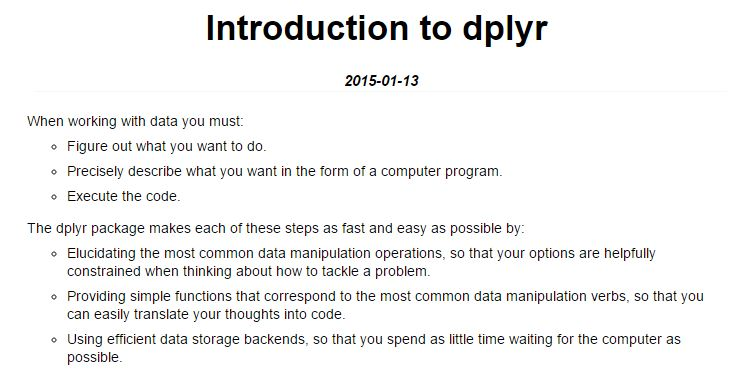
\includegraphics[width=1.15\linewidth]{images/introdplyr}

\end{figure}

		
	\end{frame}
	
	%=================================================%
	\begin{frame}
		\begin{figure}
			\centering
			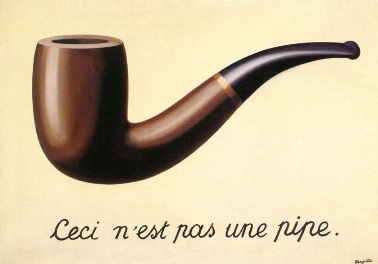
\includegraphics[width=0.99\linewidth]{images/pipe}
			
		\end{figure}
		\begin{center}
			{\huge THE $ \%>\% $ OPERATOR}
		\end{center}
		
		
		
	\end{frame}
	
	\begin{frame}
		\begin{figure}
			\centering
			
\includegraphics[width=0.99\linewidth]{images/pipe2}
			
		\end{figure}
		
	\end{frame}
	%=================================================%
	\begin{frame}[fragile]
		\frametitle{ The $\%>\%$ operator}
		\LARGE
		% - http://r2014-mtp.sciencesconf.org/file/92631
		\begin{itemize}
			\item From \textbf{magrittr} package. 
			\item Used extensively in \textbf{dplyr}.
			\item $\%>\%$ is a piping operator, and can be verbalised as ``\textit{then}".
			\item It takes the output of the left side, and uses it as the first
			argument of the function on the right side.
		\end{itemize}
	\end{frame}
	%================================================================= %
	\begin{frame}[fragile]
		\frametitle{magrittr :  the $\%>\%$ operator}
		\Large
		\begin{framed}
			\begin{verbatim}
			subset(mtcars, cyl == 6, c(mpg, wt))
			
			mtcars %>% subset(cyl == 6, c(mpg, wt))
			\end{verbatim}
		\end{framed}
		
	\end{frame}
	
	\begin{frame}
		\begin{figure}
			\centering
			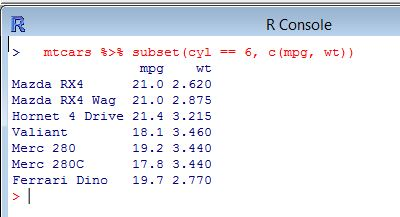
\includegraphics[width=0.99\linewidth]{images/magrittrcode01}
			
		\end{figure}
		
	\end{frame}
	%================================================================= %
	\begin{frame}[fragile]
		\frametitle{magrittr :  the $\%>\%$ operator}
		\Large
		\begin{framed}
			\begin{verbatim}
			
			summary(subset(mtcars, cyl == 6, 
			c(mpg, wt)), digits=2)
			
			mtcars %>% 
			subset(cyl == 6, c(mpg, wt)) %>% 
			summary(digits=2)
			\end{verbatim}
		\end{framed}
		
	\end{frame}
	%================================================================= %
	\begin{frame}[fragile]
		\frametitle{magrittr :  the $\%>\%$ operator}
		\Large
		\begin{framed}
			\begin{verbatim}	
			mtcars %>% 
			subset(cyl == 6, c(mpg, wt)) %>% 
			summary(digits=2)
			\end{verbatim}
		\end{framed}
		\begin{itemize}
			\item Get the mtcars data set
			\item \textbf{Then} subset it like this
			\item \textbf{Then} get the summary, with this setting
		\end{itemize}
	\end{frame}
	
	\begin{frame}
		\begin{figure}
			\centering
			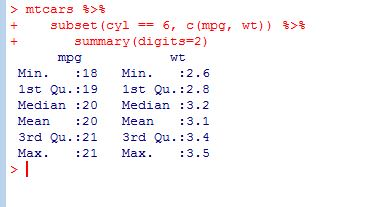
\includegraphics[width=0.99\linewidth]{images/magrittrcode02}
			
		\end{figure}
		
	\end{frame}

%================================================================= %
\begin{frame}
	\frametitle{magrittr :  the $\%>\%$ operator}
	\begin{itemize}
		\item You can use the $\%>\%$ operator with any \texttt{R} functions.
		\item The rules are simple: the object on the left hand side is passed as the first argument to the function on the right hand side. So: 
	\end{itemize}
	\begin{framed}	
		my.data $\%>\%$ \texttt{my.function} is the same as \texttt{my.function(my.data)}
		my.data $\%>\%$ \texttt{my.function(arg=value)} is the same as \texttt{my.function(my.data, arg=value)}
	\end{framed}
	
\end{frame}
%=================================================%
\begin{frame}[fragile]
	\frametitle{The $ \%>\% $ Operator}
	\Large
	\textbf{The $ \%>\% $ Operator}
	\begin{itemize}
		\item ggvis makes use of the $ \%>\% $ operator from the
		package magrittr
		\item This allows us to layer up graphics in the same
		way we would with ggplot2
		
	\end{itemize}
	
	
\end{frame}
%=================================================%
\begin{frame}[fragile]
	\frametitle{The $ \%>\% $ Operator}
	\textbf{Tube Data Example }\\ (\textit{Dr. Aimee Gott, Mango Solutions})
	%		\begin{itemize}
	%			\item The $ \%>\% $ operator passes the left hand object to the
	%			first argument of the right hand expression
	%			\item We can pass data or objects to functions in this way
	%			
	%		\end{itemize}
	
	\begin{framed}
		\begin{verbatim}
		> tubeData$Excess %>%  tapply(tubeData$Line, mean)
		
		# Bakerloo              5.047714
		# Central               5.998667
		# Circle & HamDistrict  7.166095 
		
		\end{verbatim}
	\end{framed}
	
\end{frame}
%================================================================= %
\begin{frame}
	\frametitle{magrittr :  the $\%>\%$ operator}
	\Large
	\vspace{-1cm}
	\textbf{	$ \%>\% $ in ggvis}
	\begin{itemize}
		\item With ggvis we pass "\texttt{ggvis}" objects
		\item We create the initial object by passing data to
		\texttt{ggvis()}
		\item All other functions expect a ggvis object as the
		first argument and return a ggvis object
	\end{itemize}
	
\end{frame}

%============================================================================= %
	%=======================================================================================%
	\begin{frame}[fragile]
		\frametitle{Installing dplyr}
		\large
		Straightforward \texttt{R} package installation.
		\begin{framed}
			\begin{verbatim}
			install.packages("dplyr")
			library(dplyr)
			
			# Data Set Examples
			# 1. iris
			# 2. mtcars
			
			\end{verbatim}
		\end{framed}
	\end{frame}
	%===================================================================== %
	
	\begin{frame}[fragile]
		\frametitle{iris data set}
		\Large
		\begin{framed}
			\begin{verbatim}
			> names(iris)
			[1] "Sepal.Length"
			[2] "Sepal.Width" 
			[3] "Petal.Length"
			[4] "Petal.Width" 
			[5] "Species"    
			\end{verbatim}
		\end{framed}
	\end{frame}
	%============================================================================ %
	
	\begin{frame}[fragile]
		
		\frametitle{mtcars data set}
		\Large
		\begin{framed}
		\begin{verbatim}
		> names(mtcars)
		[1] "mpg"  "cyl"  "disp" "hp"  
		[5] "drat" "wt"   "qsec" "vs"  
		[9] "am"   "gear" "carb"
		\end{verbatim}
		\end{framed}
	\end{frame}
	%===================================================================================%
	\begin{frame}[fragile]
		\frametitle{Example Data Sets}
		\large
		\begin{framed}
		\begin{verbatim}
		dim(iris)
		class(iris)
		mode(iris)
		
		dim(mtcars)
		class(mtcars)
		mode(mtcars)
		\end{verbatim}
		\end{framed}
	\end{frame}
		%================================================================================ %
		\begin{frame}
			\frametitle{Grouped operations}
			\Large
			\begin{itemize}
				
				%			\item The verbs are useful, but they become really powerful when you combine them with the idea of “group by”, repeating the operation individually on groups of observations within the dataset. 
				\item In \textbf{dplyr}, you use the \texttt{group\_by()} function to describe how to break a dataset down into groups of rows. \bigskip
				\item You can then use the resulting object in exactly the same functions as above; they’ll automatically work ``by group" when the input is a grouped structure.
			\end{itemize}
		\end{frame}
		%======================================================================================%
		\begin{frame}
			
			\frametitle{\texttt{group\_by }}
			{
			\Large
			\textbf{\texttt{group\_by}}:\\ \bigskip
		}
		\large
			Group a \textit{tbl} by one or more variables.\\ \bigskip
			
			
			\textbf{Description}\\ \bigskip
			
			Most data operations are useful done on groups defined by variables in the the dataset. \\ The
			\textbf{group\_by} function takes an existing tbl and converts it into a grouped tbl where operations are
			performed "by group".
			
		\end{frame}
		%=========================================================== %
			%===================================================================================================== %
			\begin{frame}[fragile]
				
				\frametitle{The \texttt{glimpse()} Function} 
				\Large
				\vspace{-1cm}
				\begin{itemize}
					\item dplyr also provides a function \texttt{glimpse()} that makes it easy to look at the data in a transposed view. 
					
					\item similar to the \texttt{str()} (structure) function, but has a few advantages (see \texttt{?glimpse}).
					
				\end{itemize}
			\end{frame}
			%===================================================================================================== %
			\begin{frame}[fragile]
				
				\frametitle{The \texttt{glimpse()} Function }
				\begin{figure}
					\centering
					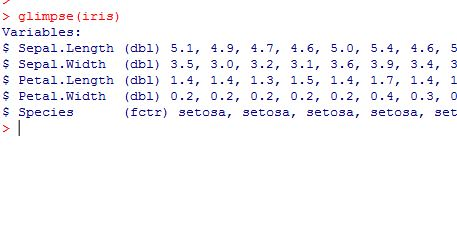
\includegraphics[width=1.2\linewidth]{images/irisglimpse}
					
				\end{figure}
				
			\end{frame}
		%==================================================================================== %
	\begin{frame}
		\frametitle{dplyr: Single Table Verbs}
		dplyr aims to provide a function for each basic verb of data manipulating:
		{
			\large
		\begin{itemize}
			\item \texttt{ filter() } (and \texttt{  slice() })
			\item \texttt{ arrange() }
			\item \texttt{ select() } (and \texttt{  rename() })
			\item \texttt{ distinct() }
			\item \texttt{ mutate() } (and \texttt{  transmute() })
			\item \texttt{ summarise() }
			\item \texttt{ sample\_n() } and \texttt{  sample\_frac() }
		\end{itemize}
	}
		%	\begin{figure}
		%\centering
		%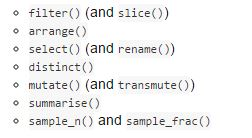
\includegraphics[width=0.7\linewidth]{images/singletableverbs}
		%
		%\end{figure}
	\end{frame}
	
	\begin{frame}
		\frametitle{Summary Statistics}
		\large
		You can use \texttt{summarise()} with aggregate functions, which take a vector of values, and return a single number.\\ \bigskip Supports functions in base \texttt{R} like \texttt{min()}, \texttt{max()}, \texttt{mean()}, \texttt{sum()}, \texttt{sd()}, \texttt{median()}, and \texttt{IQR()}.\\ \bigskip 
		\begin{itemize}
			\item 
			\texttt{n()}: number of observations in the current group
			\item 
			\texttt{n\_distinct(x)}: count the number of unique values in x.
		\end{itemize}
		
		%
		%first(x), last(x) and nth(x, n) - these work similarly to x[1], x[length(x)], and x[n] but give you more control of the result if the value isn’t present.
	\end{frame}
	%=========================================================================================%
	\begin{frame}[fragile]
		\frametitle{Grouping with the \texttt{group\_by} command}
		\large
		\vspace{-1cm}
		\begin{framed}
			\begin{verbatim}
			
			iris.sp <- group_by(iris,Species)
			class(iris.sp)
			
			summarise(iris.sp,
			    meanSL = mean(Sepal.Length), 
			    sdSL = sd(Petal.Length))
			
			\end{verbatim}
		\end{framed}
	\end{frame}
	%==================================================================== %
	\begin{frame}
		\begin{figure}
			\centering
			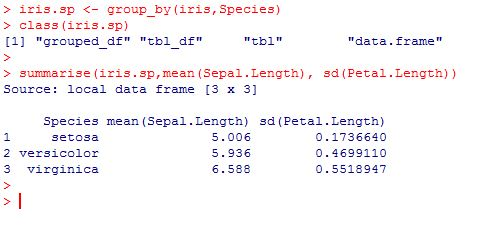
\includegraphics[width=1.15\linewidth]{images/irisgroupby}
		\end{figure}
	\end{frame}	
	%============================================================================== %
	\begin{frame}
		\begin{figure}
			\centering
			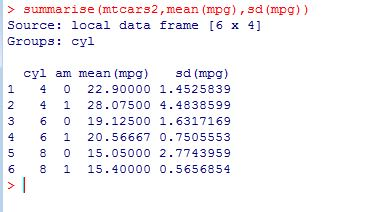
\includegraphics[width=0.9\linewidth]{images/mtcarssummarise}
			\label{fig:mtcarssummarise}
		\end{figure}
	\end{frame}
	
	
	%=========================================================================================%
	\begin{frame}
		\frametitle{Filter rows with \texttt{filter()}}
		\Large
		\vspace{-1.5cm}
		\begin{itemize}
			\item \texttt{filter()} allows you to select a subset of the rows of a data frame. 
			\item The first argument is the name of the data frame, and the second and subsequent are filtering expressions evaluated in the context of that data frame.
		\end{itemize}
		
		
		
	\end{frame}
	%=========================================================================================%
	\begin{frame}[fragile]	
		\begin{framed}
			\begin{verbatim}
			iris.vir1 <- filter(iris,Species=="virginica")
			
			# Species is Virginica OR Petal.length is 
			# greater than 3.2
			
			iris.vir2 <- filter(iris,
			    Species=="virginica" | Petal.Length >3.2)
			
			iris.vir3 <- filter(iris,
			    Species=="virginica" & Petal.Length >3.9)
			
			\end{verbatim}
		\end{framed}
	\end{frame}
	
	%=====================================================================================%
	\begin{frame}
		\frametitle{Select columns with \texttt{select()}}
		\Large
		\vspace{-1cm}
		\begin{itemize}
			\item Often you work with large datasets with many columns where only a few are actually of interest to you. 
			\item \texttt{select()} allows you to rapidly target on a useful subset using operations that usually only work on numeric variable positions.
		\end{itemize}
	\end{frame}
	
	\begin{frame}
		\frametitle{Selection Options with \texttt{select()}}
		\begin{figure}
			\centering
			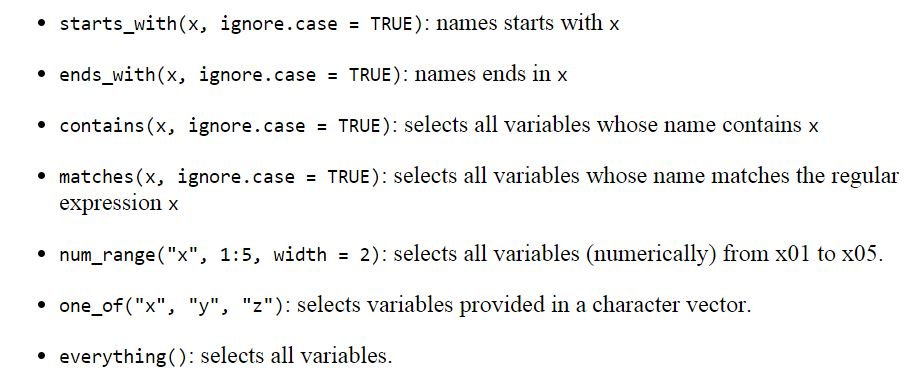
\includegraphics[width=01.25\linewidth]{images/selectoptions}
		\end{figure}
		
	\end{frame}
	%================================================================= %
	\begin{frame}
		\frametitle{Selection Options with \texttt{select()}}
		
		\begin{figure}
			\centering
			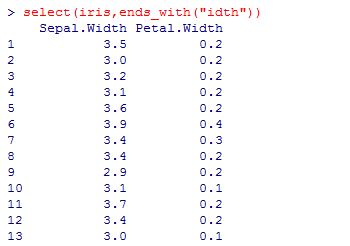
\includegraphics[width=0.89\linewidth]{images/selectendswith}
		\end{figure}
		
	\end{frame}
	
	
	\begin{frame}
		\frametitle{Selection Options with \texttt{select()}}
		
		\begin{figure}
			\centering
			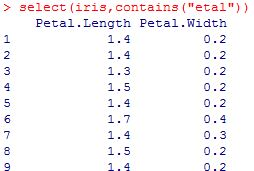
\includegraphics[width=0.69\linewidth]{images/selectioncontaints}
		\end{figure}
		
	\end{frame}
		
			%===================================================================================================== %
			\begin{frame}[fragile]
				\frametitle{The Idaho Data Set}
					
\begin{figure}
\centering
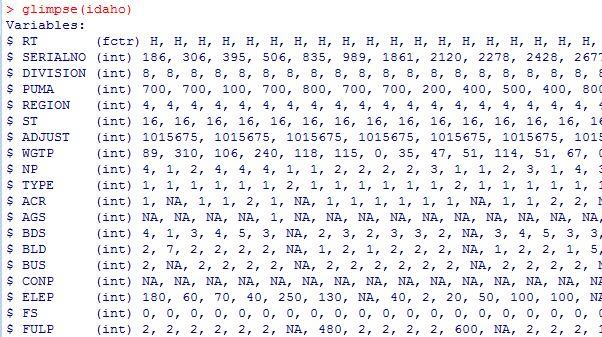
\includegraphics[width=1.2\linewidth]{images/idahoglimpse}

\end{figure}
					
				\end{frame}
				%===================================================================================================== %
				\begin{frame}[fragile]
					\frametitle{ Idaho Data Set: Multiple Selections with \texttt{select()} }
					
					Remark : Regular Expressions.
					\begin{framed}
						\begin{verbatim}
						idaho2 = select(idaho,
						    contains("AX"),
						    starts_with("FK"),
						    starts_with("SM"),
						    ends_with("SP") 
						)
						\end{verbatim}
					\end{framed}
					
				\end{frame}
				%===================================================================================================== %
				\begin{frame}[fragile]
					\frametitle{ Dropping Variables with \texttt{select()} }
					\begin{framed}
						\begin{verbatim}	
						
						# Drop variables
						select(iris, -starts_with("Petal"))
						select(iris, -ends_with("Width"))
						select(iris, -contains("etal"))
						select(iris, -matches(".t."))
						select(iris, -Petal.Length, -Petal.Width)
						\end{verbatim}
					\end{framed}
					
				\end{frame}
				

	

	%========================================================================================%
	\begin{frame}
		\frametitle{Ordering Data Sets with \texttt{arrange()}}
		\Large
		\begin{itemize}
			\item \texttt{arrange()} works similarly to \texttt{filter()} except that instead of filtering or selecting rows, it reorders them. 
			
			\item It takes a data frame, and a set of column names (or more complicated expressions) to order by.
			
			\item If you provide more than one column name, each additional column will be used to break ties in the values of preceding columns.
			
			\item Use \texttt{desc()} (or \texttt{rev()}) to order a column in descending order.
			
			%arrange(flights, desc(arr_delay))
		\end{itemize}
	\end{frame}
	%===================================================================================== %
	\begin{frame}
		\begin{figure}
			\centering
			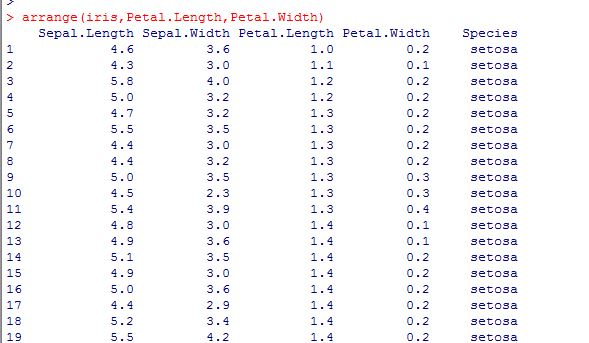
\includegraphics[width=0.97\linewidth]{images/irisarrange}
			
		\end{figure}
		
	\end{frame}
	
	%==================================================================================== %
	
	\begin{frame}
		\begin{figure}
			\centering
			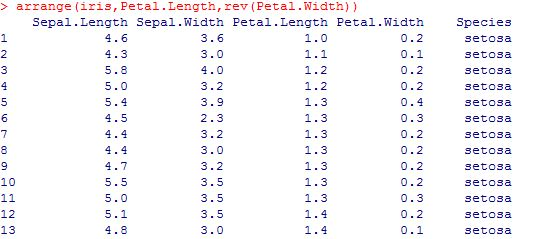
\includegraphics[width=0.97\linewidth]{images/irisarrange2}
			
		\end{figure}
		
	\end{frame}
	
	% Graphics: irisarrange
	
	
	\begin{frame}
		\frametitle{Sampling rows with \texttt{sample\_n()} and \texttt{sample\_frac()}}
		\Large
		\begin{itemize}
			\item You can use \texttt{sample\_n()} and \texttt{sample\_frac()} to take a random sample of rows, either a fixed number for \texttt{sample\_n()} or a fixed fraction for \texttt{sample\_frac()}.
		\end{itemize}
	\end{frame}
	
	\begin{frame}
		\frametitle{Sampling rows with \texttt{sample\_n()} and \texttt{sample\_frac()}}
		\Large
		
		\begin{figure}
			\centering
			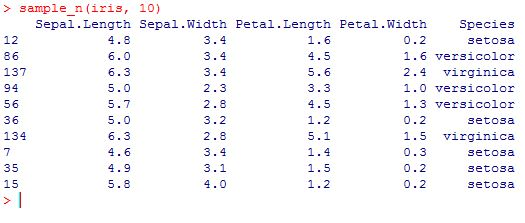
\includegraphics[width=1.07\linewidth]{images/irissample1}
		\end{figure}
		
	\end{frame}
	%------------------------------------------------------------------------------------ %
	\begin{frame}
		\frametitle{Sampling rows with \texttt{sample\_n()} and \texttt{sample\_frac()}}
		
		\begin{figure}
			\centering
			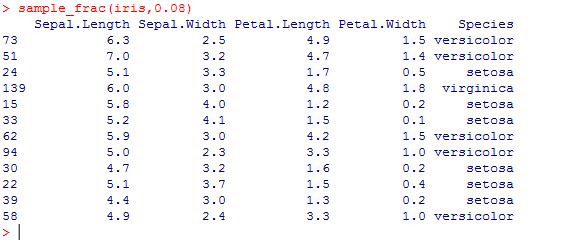
\includegraphics[width=1.07\linewidth]{images/irissample2}
		\end{figure}
		
	\end{frame}
	%------------------------------------------------------------------------------------ %
	\begin{frame}
		\frametitle{Sampling rows with \texttt{sample\_n()} and \texttt{sample\_frac()}}
		
		\begin{figure}
			\centering
			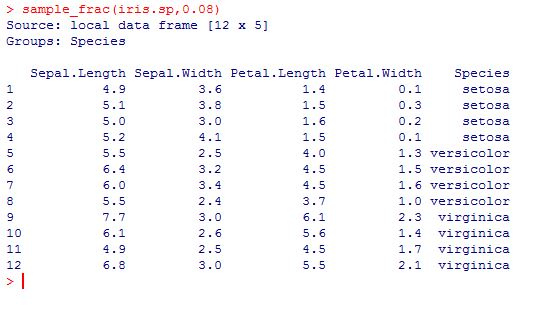
\includegraphics[width=1.07\linewidth]{images/irissample3}
		\end{figure}
		
	\end{frame}
	%=======================================================================================%
	\begin{frame}[fragile]
		\frametitle{Add new columns with \texttt{mutate()} }
		
		As well as selecting from the set of existing columns, it’s often useful to add new columns that are functions of existing columns. This is the job of \texttt{mutate()}:
		
		\begin{framed}
			\begin{verbatim}
			iris2 =  mutate(iris, 
			PW2 = log(Petal.Width), 
			PL2=sqrt(Petal.Length) )
			
			head(iris2)
			\end{verbatim}
		\end{framed}
	\end{frame}
	%================================================================================= %
	%% Graph irismutate
	\begin{frame}
		
		\frametitle{Add new columns with \texttt{mutate()} }
		\begin{figure}
			\centering
			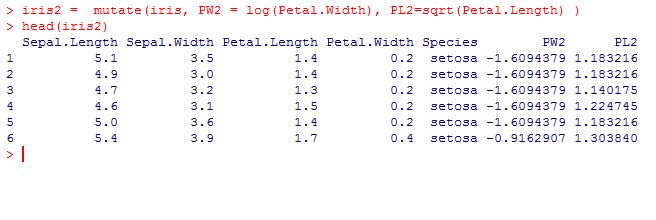
\includegraphics[width=1.2\linewidth]{images/irismutate}
			
		\end{figure}
		
	\end{frame}
	%==========================================================================%
	\begin{frame}[fragile]
		
		\frametitle{Add new columns with \texttt{mutate()} }
		\texttt{mutate} allows you to refer to columns that you just created:
		
		\begin{verbatim}
		iris3 =  mutate(iris, 
		PW2 = log(Petal.Width), 
		PL2=sqrt(Petal.Length), 
		Ratio=PL2/PW2 )
		
		head(iris3)
		\end{verbatim}
	\end{frame} 
	%================================================================== %
	\begin{frame}
		
		\frametitle{Add new columns with \texttt{mutate()} }
		\begin{figure}
			\centering
			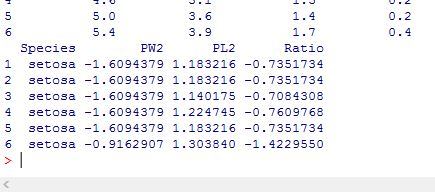
\includegraphics[width=0.9\linewidth]{images/irismutate2}
			
		\end{figure}
		
	\end{frame}
	
	
	%% Graphic irismutate2
	\begin{frame}
		\frametitle{Multiple table verbs}
		
		As well as verbs that work on a single \texttt{tbl}, there are also a set of useful verbs that work with two \texttt{tbl}s at a time: joins and set operations.
	\end{frame}
	\begin{frame}
		\frametitle{Joins}
		dplyr implements the four most useful joins from SQL:
		
		\begin{itemize}
			\item \texttt{inner\_join(x, y)}: matching x + y
			\item \texttt{left\_join(x, y)}: all x + matching y
			\item \texttt{semi\_join(x, y)}: all x with match in y
			\item \texttt{anti\_join(x, y)}: all x without match in y
		\end{itemize}
	\end{frame}
	\begin{frame}
		\begin{figure}
			\centering
			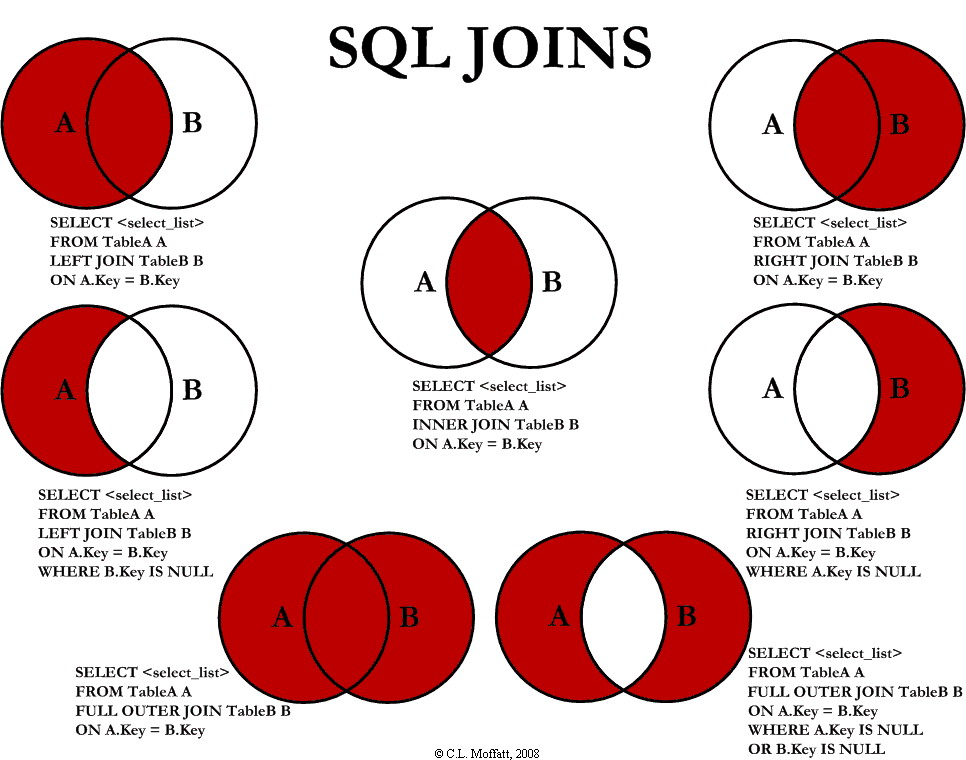
\includegraphics[width=1.00\linewidth]{images/SQLjoins}
			
		\end{figure}
		
	\end{frame}
	\begin{frame}
		\frametitle{Joins}
		Pretend data set listing country of origin for each species.
		The variables ``Species" is common to both data frames.
		\begin{figure}
			\centering
			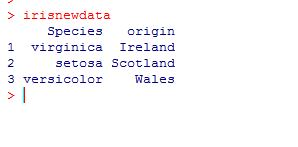
\includegraphics[width=0.7\linewidth]{images/irisnewdata}
			\caption{Second Data Frame}
			\label{fig:irisnewdata}
		\end{figure}
		
	\end{frame}
	
	\begin{frame}
		\frametitle{Joins}
		\begin{figure}
			\centering
			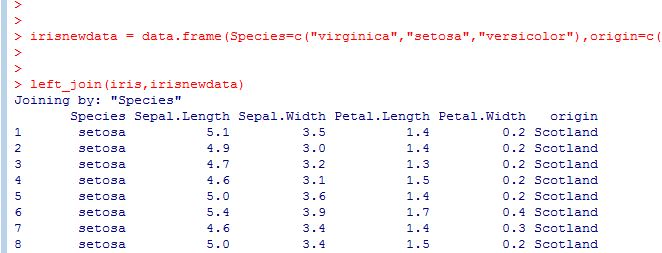
\includegraphics[width=0.97\linewidth]{images/irisjoin}
			
			\label{fig:irisjoin}
		\end{figure}
		
	\end{frame}
	%======================================================================= %
	
	\begin{frame}
		\frametitle{Set Theory Operations}
		
		dplyr implements the methods for set theory operations
		
		\begin{itemize}
			\item \texttt{intersect(x, y)}: all rows in both x and y
			\item \texttt{union(x, y)}: rows in either x or y
			\item \texttt{setdiff(x, y)}: rows in x, but not y
		\end{itemize}
	\end{frame}
	
	
\end{document}
